\documentclass{beamer}
\usepackage[utf8]{inputenc}
\usepackage[T1]{fontenc}


\title{Das neue \LaTeX-Beamer Theme der TU Dortmund}
\author{Maximilian Nöthe}
\institute[Lehrstuhl E5b \\ Fakultät Physik]{Lehrstuhl E5b \par\vspace{3pt} Fakultät Physik}
\titlegraphic{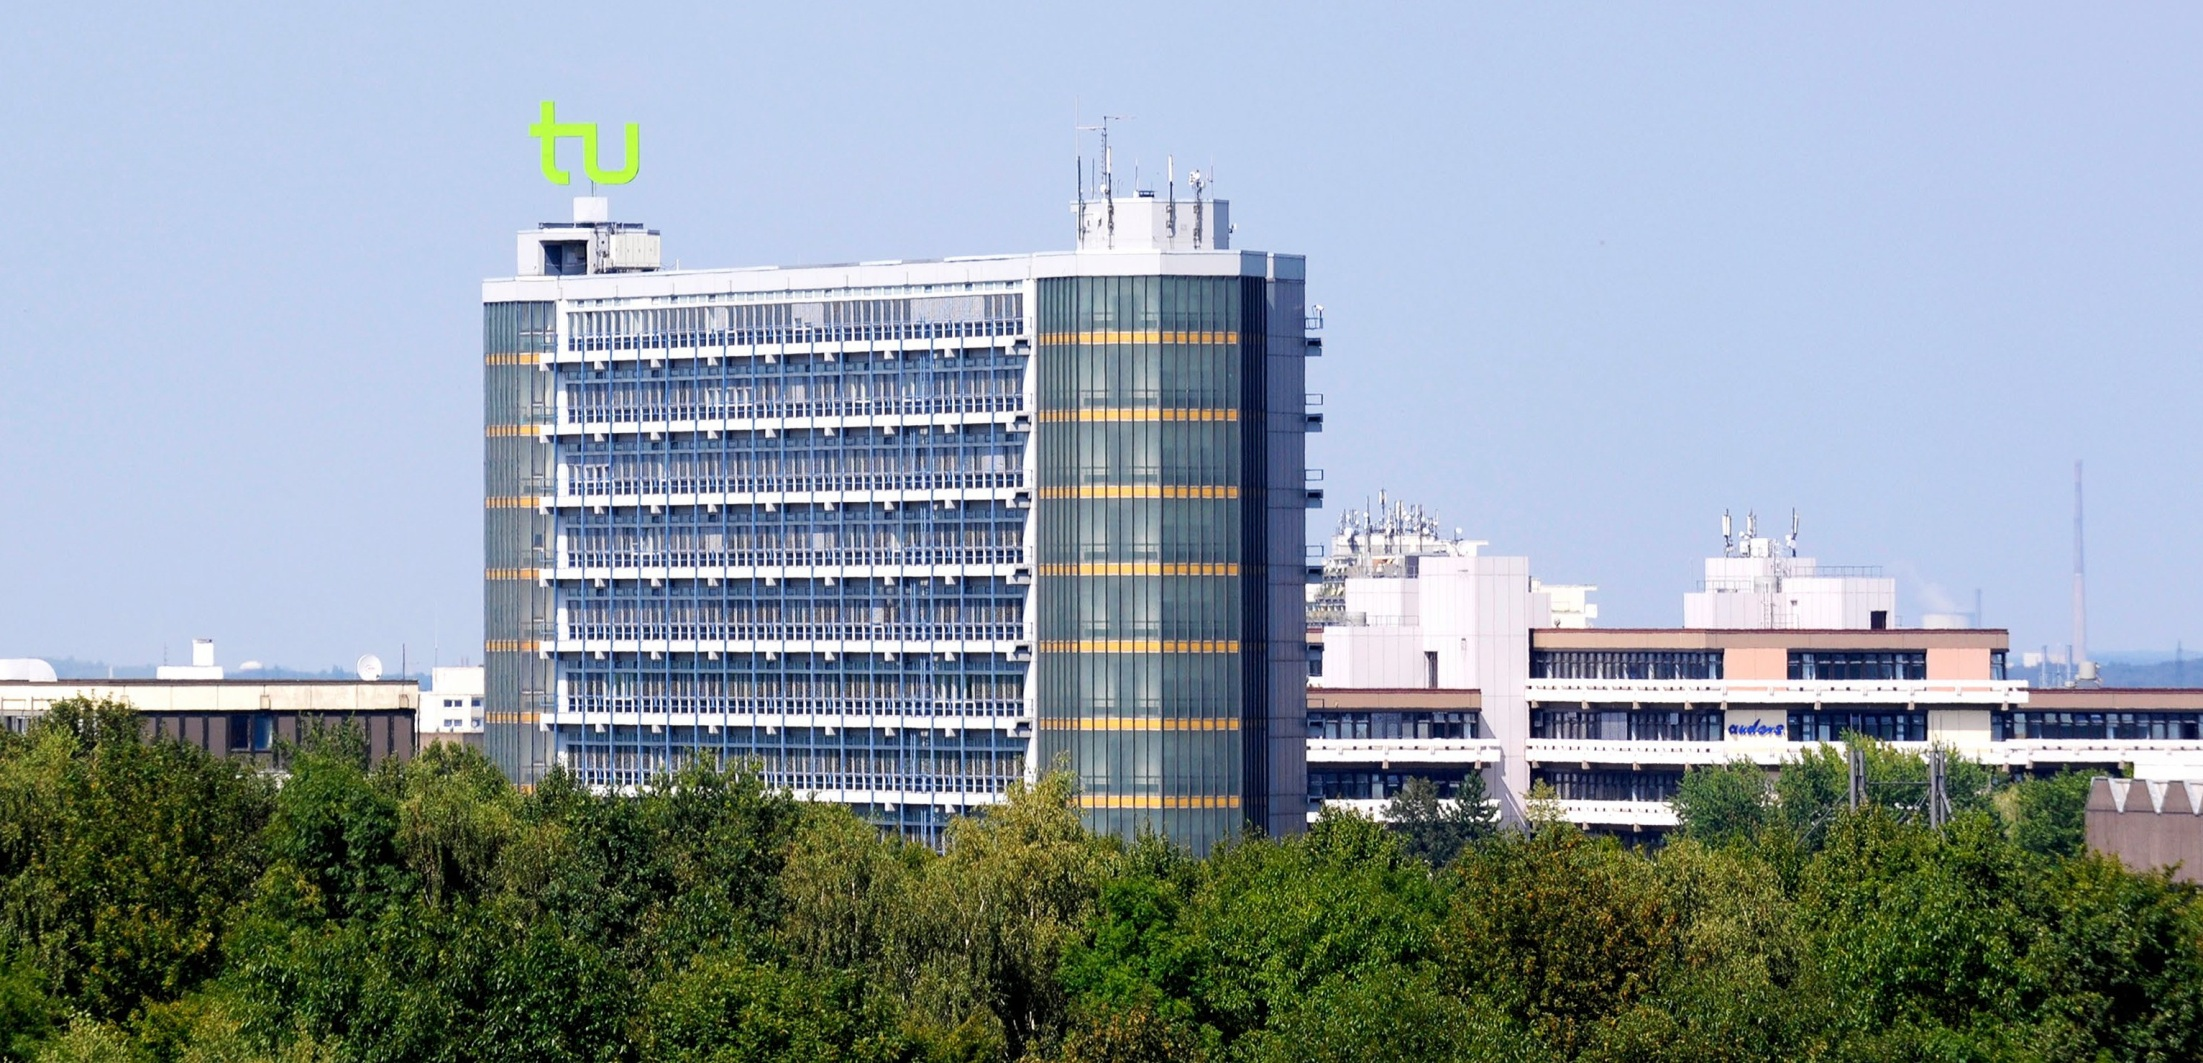
\includegraphics[height=0.7\textheight]{Title-Pic.jpg}}

\usetheme{TUDo}

\begin{document}

\begin{frame}
\setcounter{framenumber}{0}
    \titlepage
\end{frame}

\begin{frame}
    \frametitle{Einführung}
    \tableofcontents[pausesections]
\end{frame}

\section{Das Design}
\subsection{Farben und Formen}
\begin{frame}
    \frametitle{Die TU-Farbpalette}
    \begin{itemize}
        \item \textcolor{TUgreen}{TUgreen}
            \begin{itemize}
                \item \textcolor{TUdarkgreen}{TUdarkgreen}
                \item \textcolor{TUolive}{TUolive}
            \end{itemize}
        \item \textcolor{TUyellow}{TUyellow}
        \item \textcolor{TUcitron}{TUcitron}
        \item \textcolor{TUlime}{TUlime}
        \item \textcolor{TUorange}{TUorange}
    \end{itemize}
\end{frame}

\subsection{Blöcke}
\begin{frame}
    \frametitle{Blöcke}
    \begin{block}{Test}
        \begin{itemize}
            \item 1
            \item 2
        \end{itemize}
    \end{block}
\end{frame}

\section{Tolle neue Slides}
\subsection{Altes Slides aus der CD-Powerpoint}
\begin{frame}
    \begin{enumerate}
        \item Test 1
        \item Test 2
    \end{enumerate}
\end{frame}


\subsection{Viel bessere neue Templates}
\begin{frame}
    \begin{enumerate}
        \item Test 1
        \item Test 2
    \end{enumerate}
\end{frame}

\end{document}
